\section{Método proposto} \label{sec:metodo}

Nesta seção estudaremos uma estrutura em dois níveis para a complementação automática de consulta tolerante a erros que usa o algoritmo \textit{ICPAN} no primeiro nível e pesquisa tanto sequencial quanto binária no segundo nível. Para validar a ideia de busca binária no segundo nível utilizamos o ICPAN no primeiro por ser relativamente mais fácil de implementá-lo em comparação com o BEVA, que será utilizado no primeiro nível futuramente neste trabalho. O primeiro nível serve como um filtro principal que seleciona candidatos à resposta para serem processados no segundo nível, que por sua vez determina quais desses candidatos são qualificados como resposta final.

O intuito dessa abordagem é reduzir o uso de memória e ao mesmo tempo manter o desempenho quanto ao tempo de processamento da consulta. Os sistemas de busca podem se beneficiar dessa redução pois ela possibilita diminuir os custos com memória mantendo o mesmo conjunto de dados, ou então pode permitir o aumento do conjunto de dados sem que haja um grande impacto na quantidade de memória usada pelo método.

Seja $\mathcal{D}$ a base de dados considerada nos parágrafos a seguir, composta pelos seguintes itens: \textit{\{``insects, integer, integral, integrity, intellect, intelligent, invest, invested, investigate, telepathic, telepathy, telephone, telephoto, teleport, teleprompter''\}}. Atribuímos um valor de $id$ a cada item, partindo do número $0$, como é possível observar na tabela de itens da Figura~\ref{fig:index_structure}. A etapa de indexação considera que todos os itens estão ordenados em ordem lexicográfica crescente, e para que os exemplos fiquem mais simples cada item contém apenas uma palavra.
 
\subsection{Indexação} 
\label{sec:indexing}
Seja $w$ a cadeia de caracteres de um item, e $|w|$ o tamanho da cadeia, e $w[i]$ uma indicação do $i$-ésimo caractere de $w$, começando a partir de $1$. Assim, $w[i..j]$ representa uma subcadeia de caracteres de $w$ começando na $i$-ésima posição e terminando na $j$-ésima. Consideramos também que se $j > |w|$, então $w[i..j] = w$, e também que $w[i..]$ representa a subcadeia que começa no $i$-ésimo caractere, e termina no último caractere de $w$. Sendo assim, para $w = ``sapato"$, $w[3..27] =  ``pato"$ e $w[4..] = ``ato''$, por exemplo.  

 
 \begin{figure} [ht]
    \centering
    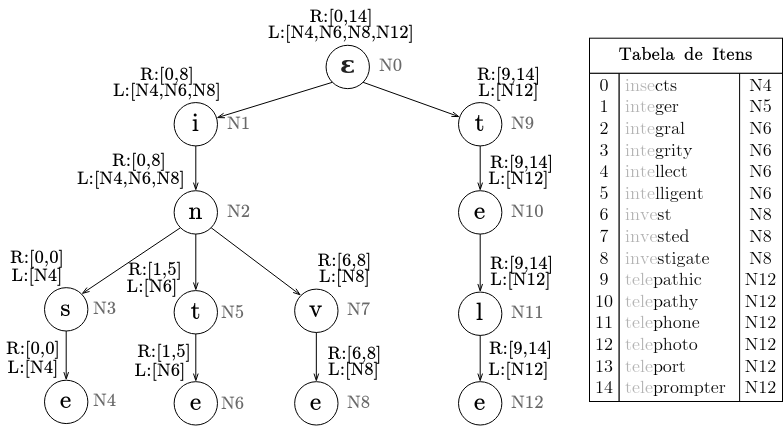
\includegraphics[width=0.94\textwidth]{figures/index-structure.png}
    \caption{Árvore \textit{Trie} com os prefixos de tamanho $\lambda = 4$ indexados, na qual cada possui intervalos $R$ de \textit{ids} e listas $L$ de nós folha dentre os seus descendentes.}
    \label{fig:index_structure}
\end{figure}

 
Como parte da implementação da estrutura proposta, indexamos as descrições textuais dos itens em uma árvore \textit{Trie} $\mathcal{T}$ mantida em memória. Seja também $\lambda$ a altura máxima permitida para $\mathcal{T}$, considerando que o nível do nó $\epsilon$ (nó $N0$ na Figura~\ref{fig:index_structure}) é igual a $0$. Dessa forma, o nó $N7$ tem altura igual a $3$, por exemplo. Para cada cadeia $w$ de um item, inserimos em $\mathcal{T}$ apenas o prefixo $Prefixo_{\lambda}(w)$, onde $Prefixo_{\lambda}(s) = s[1..\lambda]$ é uma função que retorna os $\lambda$ primeiros caracteres da cadeia $s$ passada como parâmetro.

Cada nó $n$ em $\mathcal{T}$ contém um caractere $n.caractere$, um número de identificação $n.id$, e a sua altura $n.altura$ correspondente na árvore (sendo a altura do nó $\epsilon$ igual a 0). Também possui um intervalo $n.R = [menor, maior]$ no qual $menor$ e $maior$ representam respectivamente o menor e o maior $id$ dos itens em $\mathcal{T}$ que compartilham o mesmo prefixo $p_{n}$ obtido ao caminhar partindo do nó $\epsilon$ até $n$. Esse intervalo é análogo à lista invertida mencionada no fim da seção~\ref{sec:icpan_algorithm_description}. Para uma subárvore com raiz no nó $n$, todos os itens nessa subárvore irão compartilhar o mesmo prefixo $p_{n}$. Objetivando a simplicidade, iremos nos referir a $n$ pelo seu prefixo $p_{n}$ correspondente de forma intercambiável, assim como foi feito na seção~\ref{sec:trie}. 

Por fim, cada nó $n$ possui uma lista $n.L$ que contém todos os nós-folha de sua subárvore. Quando o próprio $n$ é uma folha, não possui subárvore, então a lista conterá apenas o próprio $n$, ou seja, $n.L = [n.id]$.

A Figura~\ref{fig:index_structure} mostra uma \textit{Trie} $\mathcal{T}$ após a indexação dos $\lambda = 4$ primeiros caracteres de cada item em $\mathcal{D}$. Também mantém-se uma estrutura de dicionário $\mc{H}$, representada pela ``Tabela de Itens'', que mapeia o valor do \textit{id} de um item ao texto do restante da sua descrição, ou seja, $w[5..]$ (texto após o 4º caractere).

Essa estrutura é utilizada para reconstruir a descrição completa de um item a partir de qualquer nó de prefixo \textit{p}. Apesar de a Figura~\ref{fig:index_structure} mostrar o texto completo de cada item, os $4$ primeiros caracteres em cinza claro são na verdade obtidos ao caminhar por $\mathcal{T}$. Para possibilitar essa reconstrução, também guardamos em $\mc{H}$ o $id$ do nó correspondente ao prefixo $Prefixo_{\lambda}(w)$ do item. Supondo por exemplo a reconstrução de ``\textit{investigate}'', com $id=7$ em $\mc{H}$, basta processar o prefixo $p$ do nó $N8$, que é \textit{p = ``inve''}, como mostra a Figura~\ref{fig:index_structure}, e então concatenar $p$ com ``\textit{stigate}'', que é o conteúdo presente em $\mc{H}$ para a chave $id=7$.

\begin{algorithm}[ht]
\caption{Construção de um índice Trie $\mc{T}$ a partir de sugestões de consultas de uma base $\mc{D}$}\label{alg:dataset_indexing}
\begin{algorithmic}[1]
\Function{ConstruirIndiceTrie}{$\mc{D}, \mc{H}, \mc{T}$}
    \For{$Q \in \mc{D}$}
        \State $item.noPrefixo \leftarrow inserirPrefixo(\mc{T}, Prefixo_{\lambda}(Q.texto), Q.id)$
         \If{$|Q.texto| < \lambda$}
            \State $item.restante \leftarrow \epsilon$
         \Else{}
            \State $item.restante \leftarrow Q.texto[(\lambda + 1)..]$
         \EndIf
         
         \State $\mc{H}[Q.id] \leftarrow item$
    \EndFor
    \State $construirListasDeFolhas(\mc{T})$
\EndFunction
\end{algorithmic}
\end{algorithm}

O Algoritmo~\ref{alg:dataset_indexing} descreve a construção de um índice Trie a partir de uma base de sugestões de consulta. Esse algoritmo tem como parâmetro: $\mc{D}, \mc{H}, \mc{T}$, os quais representam, respectivamente, a base de dados com as sugestões de consulta que serão indexadas, a estrutura de dicionário mencionada anteriormente, e a árvore Trie ainda vazia. Esse algoritmo assume que os itens da base $\mc{D}$ estão em ordem lexicográfica crescente. O laço de repetição da linha 2 define o procedimento feito para cada sugestão de consulta $Q$ da base $\mc{D}$. Na linha 3, chama-se a função $inserirPrefixo$ (que será detalhada a seguir), a qual insere o prefixo $Prefixo_{\lambda}(Q.texto)$ (primeiros $\lambda$ caracteres do texto da sugestão de consulta) na Trie, e retorna o nó da Trie referente ao prefixo inserido. Então, esse nó é atribuído ao atributo $noPrefixo$ do $item$. Na linha 4, há uma condição para verificar se o tamanho do texto de $Q$ é menor que $\lambda$. Se for, então o atributo $restante$ do $item$ recebe o valor de texto vazio $\epsilon$, na linha 5. Senão, recebe o valor do restante do texto de $Q$ após o $\lambda$-ésimo caractere, na linha 7. Com o item já montado, associa-se a chave $Q.id$ com o $item$ no dicionário $\mc{H}$ na linha 8, e o laço de repetição segue para a próxima sugestão de consulta de $\mc{D}$ se houver. Após o termino do laço, chama-se a função $construirListasDeFolhas$ na linha 9. Essa função itera sobre cada nó $n$ da Trie  $\mc{T}$, preenchendo as listas $n.L$ de cada nó, as quais contêm todos os nós-folha com raiz em $n$.


\begin{algorithm}[H]
\caption{Inserção de um prefixo de sugestão de consulta em $\mc{T}$}\label{alg:append_prefix_trie}
\begin{algorithmic}[1]
\Function{inserirPrefixo}{$\mc{T}, prefixo, id$}
    \State $raiz \leftarrow obterRaiz(\mc{T})$d
    \State $n \leftarrow raiz$
    \State $raiz.R.maior = id$
    \For{$caractere \in prefixo$}
        \State $n \leftarrow n.inserirFilho(caractere, id)$
    \EndFor
    \State $n.marcadoFolha \leftarrow Verdadeiro$
    \State $n.L.inserir(id)$
    \State \textbf{return} $n$
\EndFunction
\end{algorithmic}
\end{algorithm}

O Algoritmo~\ref{alg:append_prefix_trie} descreve a inserção de um prefixo de sugestão de consulta (o qual pode na verdade ser a consulta inteira). Esse algoritmo tem como parâmetro: $\mc{T}, prefixo, id$, os quais representam a árvore Trie, o prefixo de sugestão de consulta, e a identificação numérica da consulta, respectivamente. Na linha 4, atualiza-se o valor $maior$ do intervalo $raiz.R = [menor, maior]$ para ser igual ao $id$ da sugestão de consulta que está sendo inserida. Então, cada caractere do $prefixo$ (linha 5) é inserido na Trie um a um na (linha 6). A cada inserção, o nó $n$ é atualizado com último nó que foi inserido ou apenas percorrido (caso todo o caminho já exista na árvore). Após essas inserções, na linha 8 o nó $n$ é marcado como folha. Por fim, o $id$ da sugestão de consulta é inserido na lista $L$ do nó $n$ na linha 9 e a função retorna $n$ na linha 10. 

\subsection{Algoritmo Geral da Abordagem em Dois Níveis}
\label{sec:general_two_level_algorithm}
% Esta premissa descrita a seguir não é 100% correta. Percebi no dia 26-05-2021 enquanto escrevia aqui que, com a implementação do conjunto de folhas virtuais, é possível computar nós ativos para os lambda+tau primeiros caracteres de p, ou para p inteiro caso |p| <= lambda + tau. Creio que vale a pena explorar essa premissa melhorada para a publicação do artigo.
Como descrito na seção~\ref{sec:indexing}, somente os $\lambda$ primeiros caracteres de cada sugestão de consulta da base são indexados na Trie. Então, devido a esse fato, temos a premissa de que somente os $\lambda$ primeiros caracteres de um prefixo de consulta $p$ devem ser considerados na computação do conjunto de nós ativos. Com tal conjunto computado, cada nó é visitado, e recupera-se sua lista de nós-folha. Para cada uma das listas invertidas desses nós-folha, é possível realizar a busca sequencial apresentada na seção~\ref{sec:sequential_search}. 

\begin{algorithm}[H]
\caption{Algoritmo geral do processamento em dois níveis}\label{alg:general_two_level}
\begin{algorithmic}[1]
\Function{processarConsultaDoisNiveis}{$\mc{T}, p, \tau$}
    \State $sugestoes \leftarrow \emptyset$
    \State $nosAtivos \leftarrow computarNosAtivos(\mc{T}, Prefixo_{\lambda}(p), \tau)$ \Comment{Primeiro Nível}
    \For{$n \in nosAtivos$} \Comment{Segundo Nível (até a linha 6)}
        \For{$n_{folha} \in n.L$}
            \State $sugestoes \leftarrow sugestoes \cup buscaSequencial(p, n_{folha}.R, \tau)$
        \EndFor
    \EndFor
    \State \textbf{return} $sugestoes$
\EndFunction
\end{algorithmic}
\end{algorithm}

O Algoritmo~\ref{alg:general_two_level} é uma representação geral da abordagem em dois níveis para o problema de CATE. Ele tem como parâmetros $\mc{T}, p$ e $\tau$, os quais representam um índice Trie, um prefixo de consulta, e o limiar de erros de digitação, respectivamente. O algoritmo tem início na linha 2, inicializando uma o conjunto de resposta $sugestoes$, que conterá no fim da execução as sugestões de consultas com prefixos similares a $p$ considerando uma diferença de distância de edição de no máximo $\tau$. Na linha 3, é executada a função $computarNosAtivos$, que computa o conjunto de nós ativos da Trie $\mc{T}$ para o prefixo $Prefixo_{\lambda}(p) = p[1..\lambda]$ considerando o limiar $\tau$. O algoritmo utilizado para tal computação pode ser, em tese, qualquer um baseado em processamento de nós ativos de árvores Trie, como por exemplo o ICAN, ICPAN, ou BEVA. O conjunto final de nós ativos é armazenado na variável $nosAtivos$. Essa etapa caracteriza o primeiro nível. 

A linha 4 caracteriza o início do processamento do segundo nível. Nela há um laço de repetição que itera sobre cada nó ativo do conjunto $nosAtivos$, e na linha 5, há outro laço que itera sobre cada nó folha com raiz em $n$. Então, na linha 6, a função $buscaSequencial$ determina quais dentre as sugestões de consultas referenciadas pelo intervalo $n_{folha}$ são respostas válidas, e então essas sugestões são unidas com o conjunto final de respostas. Por fim, na linha 7 o conjunto de respostas é retornado.



\subsection{Primeiro nível}
\label{sec:first-level}

O algoritmo de busca utilizado no primeiro nível será o ICPAN, proposto por Li et al. Como descrito na seção~\ref{sec:ref_teorico} o ICPAN utiliza um algoritmo incremental que calcula os prefixos sem elhantes a um prefixo consultado, tolerando uma quantidade erros de digitação previamente definida como o limite de distancia de edição $\tau$. Uma característica desse algoritmo é a ``ativação'' de nós da \textit{Trie} que correspondem a um prefixo que pode ser obtido considerando erros no prefixo consultado.

Ao considerar a utilização do ICPAN no primeiro nível, é preciso atentar para dois pontos: (1) uma vez que o primeiro nível serve apenas como filtro para o processamento do segundo nível, o algoritmo computará nós (pivô) ativos referentes a prefixos semelhantes a uma parte $p[1..\lambda]$ de um prefixo de consulta $p$, e não semelhantes a $p$ por completo. Esse conjunto será referido como $\Psi_{p[1..\lambda]}$ daqui em diante; (2) uma premissa da concepção original desse algoritmo é que todo o texto da sugestão de consulta estará indexado na Trie, o que não acontece na abordagem em dois níveis.

Dessa maneira, o propósito original de utilização dos nós ativos foi modificado. Alguns nós importantes para o processamento no segundo nível acabam sendo desativados durante o processamento incremental do ICPAN, e deixam de estar presentes em $\Psi_{p[1..\lambda]}$. A partir dessa situação observamos em nossa pesquisa que o conteúdo do conjunto $\Psi{p[1..\lambda]}$ resultante da computação original do ICPAN \textit{não é suficiente para resolver completamente o problema de CATE na abordagem em dois níveis}. 

\subsubsection{Conjunto de Nós Folha Virtuais Ativos}
\label{sec:virtual_leaves_node-set}

Devido ao problema de nós desativados mencionado acima, faz-se necessário um mecanismo que preserve esses nós ativos importantes para que eles também estejam no conjunto final de nós ativos de $p[1..\lambda]$. O mecanismo proposto neste trabalho para resolver esse problema consiste em computar, simultaneamente ao conjunto de nós ativos $\Psi$ do ICPAN, um conjunto $\psi$ de ``nós folha virtuais ativos'' auxiliar que manterá esses nós importantes que acabariam sendo desativados durante o processamento incremental dos nós ativos. 

Como foi descrito na seção~\ref{sec:icpan_algorithm_description}, a computação do conjunto de nós ativos para um prefixo de consulta $p = c_{1}c_{2}c_{3}...c_{n}$ ocorre de forma incremental: inicializa-se um conjunto com os nós ativos para a cadeia vazia $\epsilon$, representado por $\Psi_{\epsilon}$; então, quando o primeiro caractere $c_{1}$ de $p$ é processado, os nós de $\Psi_{\epsilon}$ e alguns de seus descendentes são examinados e, dependendo de algumas condições, são inseridos no conjunto de nós ativos para a cadeia de caracteres $c_{1}$, representado por $\Psi_{c_{1}}$; quando o caractere $c_{2}$ é processado, analogamente ao passo anterior os nós de $\Psi_{c_{1}}$ e alguns de seus descendentes são examinados para determinar se serão inseridos no conjunto de nós ativos para a cadeia de caracteres $c_{1}c_{2}$, representado por $\Psi_{c_{1}c_{2}}$. Esse processo continua até que se obtenha o conjunto $\Psi_{p} = \Psi_{c_{1}c_{2}c_{3}...c_{n}}$, o qual será chamado de ``conjunto final''. Os conjuntos gerados antes do final serão chamados ``conjuntos intermediários''.

Na abordagem de dois níveis proposta neste trabalho, em que apenas os $\lambda$ primeiros caracteres das sugestões de consulta são indexados, a computação de nós ativos ocorre somente até o conjunto intermediário $\Psi_{p_[1..\lambda]}$, ou seja, o conjunto de nós ativos para os $\lambda$ primeiros caracteres de $p$. No entanto, existem alguns nós em especial que só serão encontrados no conjunto final, quando o processo continua após o $\lambda$-ésimo caractere. Quando se processa somente $p[1..\lambda]$, esses nós em especial são inseridos em alguns dos conjuntos intermediários, como em $\Psi_{c_1c_2}$, mas já não permanecem mais a partir de $\Psi_{c_1c_2c_3}$ em diante, por exemplo, e não estarão inclusos no conjunto final $\Psi_{p[1..\lambda]}$ do primeiro nível, e também não estarão inclusos no conjunto $\Psi_{p_[1..\lambda]}$, que é utilizado para o processamento do segundo nível. A consequência desse problema é que algumas sugestões de consulta que só poderiam ser obtidas através desses nós não são analisadas no segundo nível, e então o algoritmo em dois níveis proposto deixa de trazer todos os resultados que deveria. Uma vez que ainda há texto do prefixo de consulta após o $\lambda$-ésimo caractere para considerar no cálculo de distância de edição que determinar se uma sugestão deve ser sugerida, esses nós precisam ser mantidos de alguma forma para também serem analisados no segundo nível.

Denominamos esses nós que acabam ``se perdendo'' durante a computação do conjunto de nós ativos como ``nós folha virtuais ativos''. Seja $\Psi_{c_{x}}$ o conjunto de nós ativos para um prefixo de consulta $p_{x} = c_1c_2...c_{x}$ digitado anteriormente, $c_{x+1}$ um novo caractere digitado pelo usuário que resulta no novo prefixo de consulta $p_{x+1} = c_1c_2...c_{x}c_{x + 1}$. Diante disso, é necessário examinar cada nó de $\Psi_{c_{x}}$ e alguns de seus descendentes para computar o conjunto $\Psi_{c_{x + 1}}$. Um nó é considerado como folha virtual ativo se, após examiná-lo em $\Psi_{c_{x}}$, nenhum nó é inserido ou atualizados em $\Psi_{c_{x + 1}}$, pois não foi possível realizar nenhuma substituição ou inserção de acordo com as regras de manutenção de conjunto de nós ativos do ICPAN definidas na seção~\ref{sec:icpan_algorithm_description}. O nome ``nó folha virtual ativo'' se dá pelo fato de que esse nó ativo, mesmo não sendo um nó folha de fato na Trie, não gera nenhuma atualização do conjunto $\Psi_{c_{x + 1}}$ e também não vai gerar atualizações nos próximos conjuntos (quando houver).

Para manter os nós folha virtuais ativos encontrados durante a computação dos conjuntos de nós ativos, nós projetamos uma modificação no algoritmo de manutenção dos nós ativos do ICPAN para manter também um conjunto $\psi$ de nós folha virtuais ativos, representada no Algoritmo~\ref{alg:compute_active_and_virtual_leaf_nodes}. O algoritmo tem como entrada os parâmetros $\Psi_{p_x}, \psi$ e $\tau, c_{x+1}$, os quais representam, respectivamente, o conjunto de nós ativos já computado para o prefixo digitado anteriormente, o conjunto de nós folha virtuais ativos, o limite de tolerância de erros de digitação, e o novo caractere do prefixo de consulta a ser processado. Na linha 2 o conjunto de nós ativos para o prefixo atualmente processado é criado, inicializado como um conjunto vazio. Na linha 3, a variável $ativaFolhasVirtuais$ recebe o resultado de uma expressão booleana, que verifica se o tamanho do prefixo atual é maior que a diferença entre o limite $\lambda$ de altura do primeiro nível e o limite de tolerância de erros $\tau$. 

O resultado dessa expressão controlará se o conjunto $\psi$ será atualizado ou não. Sem esse controle, o conjunto $\psi$ acabará armazenando uma quantidade muito grande de nós, o que prejudicará o desempenho de processamento do segundo nível. Se $\lambda = 5$ e $\tau = 3$ por exemplo, ao considerar qualquer prefixo da Trie com tamanho igual a $5$, ao aplicar a operação de $\tau = 3$ deleções, a subcadeia resultante terá obrigatoriamente tamanho $\lambda - \tau = 2$. Então, a heurística de ativação do conjunto $\psi$ se baseia nesse limite de $\tau$ deleções. 

Na linha 4 define-se o laço de repetição de iteração sobre todas tuplas de $\Psi_{p_x}$. Na linha 5 é chamada a função $processarNoComICPAN$, que analisa o nó ativo presente na $tupla$ e alguns de seus descendentes de acordo com o algoritmo ICPAN apresentadas na seção~\ref{sec:icpan_algorithm_description}, além de atualizar (ou não) o conjunto de nós ativos atual $\Psi_{p_{x+1}}$. Para possibilitar a atualização do conjunto $\psi$, foi necessário modificar essa função originalmente utilizada no método ICPAN, para que ela passasse a retornar um valor booleano indicando se houve alguma alteração no conjunto $\Psi_{p_{x+1}}$. Esse valor é atribuído à variável $gerouAtualizacao$. Na linha 6 é verificado se o nó da $tupla$ não gerou atualização no conjunto $\Psi_{p_{x+1}}$ e se o conjunto $\psi$ deve ser atualizado. Se a expressão for verdadeira, então o conjunto $\psi$ é atualizado na linha 7. Por fim,. na linha 8 retorna-se uma tupla contendo os conjuntos $\Psi_{p_{x+1}}, \psi$.

\begin{algorithm}[t]
\caption{Computação incremental de nós ativos e nós folha virtuais }\label{alg:compute_active_and_virtual_leaf_nodes}
\begin{algorithmic}[1]
\Function{computarNosAtivosIncrementalmente}{$\Psi_{p_x}, \psi, \tau, c_{x+1}$}
    \State $\Psi_{p_{x+1}} \leftarrow \emptyset$
    \State $ativaFolhasVirtuais \leftarrow |p_{x+1}| > (\lambda - \tau)$
    
    \For{$tupla \in \Psi_{p_x}$}
        \State $gerouAtualizacao \leftarrow processarNoComICPAN(tupla, c_{x+1}, \Psi_{p_{x+1}})$
        
        \If{$\neg{gerouAtualizacao} \land ativaFolhasVirtuais$}
            \State $\psi \cup \{tupla\}$
        \EndIf
    \EndFor
    
    \State \textbf{return} $\Psi_{p_{x+1}}, \psi$
\EndFunction
\end{algorithmic}
\end{algorithm}

\subsubsection{Computação de Nós Ativos no Primeiro Nível}
\label{sec:first_level_active_node_set_computation}

% Seja $p$ um prefixo consultado pelo usuário. Considerando que $p[1..\lambda]$ é uma sub-cadeia de caracteres de $p$ que vai do 1º até o $\lambda$-ésimo caractere, e que $p[1..\lambda] = p$ se $|p| \leq \lambda$, nós processamos a subcadeia $p[1..\lambda]$ na linha $3$ com o algoritmo ICPAN caractere a caractere, de acordo com os passos do algoritmo descritos na seção~\ref{sec:second_level}. Após terminar essa etapa obtemos um conjunto $\Psi_{p[1..\lambda]} = \{ \langle n, \xi_{n}^{p[1..\lambda]}, m_{i}, \xi_{n}^{p_{i}} \rangle \}$ de \textit{nós pivô ativos de} $p[1..\lambda]$. Se $|p| \leq \lambda$ consideramos que $p$ é uma consulta ``comum'', e então realizamos o processamento caractere a caractere padrão do ICPAN para obter a resposta na linha $5$. No entanto, quando $|p| > \lambda$, é necessário dividir o processamento em dois níveis.

Estabelecida a implementação do conjunto de nós folha virtuais ativos, é possível seguir para a computação do conjunto de nós ativos do primeiro nível, os quais serão utilizados como filtro para o segundo nível, como descrito na seção~\ref{sec:general_two_level_algorithm}. Ao fim desse processo os conjuntos $\Psi_{p[1..\lambda]}$ e $\psi$ terão sido computados (para os $\lambda$ primeiros caracteres de um prefixo de consulta $p$), e a união $\Psi_{p_[1..\lambda]} \cup \psi$ determina o ``conjunto final'' $\mc{F}$ que será de fato utilizado no segundo nível. 

\begin{algorithm}[H]
\caption{Computação de nós ativos para o primeiro nível}\label{alg:compute_first_level_nodes}
\begin{algorithmic}[1]
\Function{computarNosAtivos}{$\mc{T}, p, \tau$}
    \State $raiz \leftarrow obterRaiz(\mc{T})$
    \State $\Psi = \{ \langle raiz, 0, \epsilon, 0 \rangle \}$
    \State $\psi = \emptyset$
    
    \For{$caractere \in Prefixo_{\lambda}(p)$}
        \State $\Psi, \psi \leftarrow computarNosAtivosIncrementalmente(\Psi, \psi, \tau, caractere)$
    \EndFor
    \State $\mc{F} \leftarrow \Psi \cup \psi$
    \State \textbf{return} $\mc{F}$
\EndFunction
\end{algorithmic}
\end{algorithm}

O Algoritmo~\ref{alg:compute_first_level_nodes} descreve esse procedimento, e tem como parâmetros $\mc{T}, p$ e $\tau$ que representam, respectivamente, o índice Trie, o prefixo de consulta, e o limiar de erros de edição tolerado. Na linha 2, o nó raiz da Trie é obtido. Na linha 3, o conjunto de nós ativos é inicializado com o nó raiz. Nesse momento, esse conjunto representa o conjunto $\Psi_{\lambda}$ de nós ativos para a cadeia vazia de caracteres. Esse conjunto será sobrescrito algumas vezes no decorrer do algoritmo, e no fim será representará o conjunto $\Psi_{p[1..\lambda]}$ de nós ativos para $p[1..\lambda]$. Na linha 4 o conjunto $\psi$ de nós folha virtuais ativos é inicializado como vazio. Então, na linha 5 define-se um laço de repetição para iterar sobre os $\lambda$ primeiros caracteres de $p$. Na linha 6 é chamada a função $computarNosAtivosIncrementalmente$, a qual foi descrita anteriormente na seção~\ref{alg:compute_active_and_virtual_leaf_nodes}. Os conjuntos retornados pela função sobrescrevem as variáveis $\Psi$ e $\psi$. Já na linha 7 atribui-se a união entre o conjunto $\Psi$ de nós ativos (que nesse momento representa o conjunto $\Psi_{p[1..\lambda]}$) e o conjunto $\psi$ à $\mc{F}$, que é retornada pela função na linha 8 a seguir.


% \begin{algorithm}[ht]
% \caption{Complementação de consultas tolerante a erros em dois níveis}\label{alg:2-level}
% \begin{algorithmic}[1]
% \Function{processarConsulta}{$p$}
%     \State $resultados \gets \emptyset$
%     \State $\Psi_{p[1..\lambda]} \gets processarConsultaComICPAN(p[1..\lambda])$  \Comment{Nós pivô ativos para $p[1..\lambda]$}
%     \If{$|p| < \lambda$}
%         \State \textbf{return} $recuperarResultadosICPAN(\Psi_{p[1..\lambda]})$
%     \EndIf
%     \For{$\langle n, \xi_{n}^{p[1..\lambda]}, m_{i}, \xi_{n}^{p_{i}} \rangle \in \Psi_{p[1..\lambda]} $}
%         \If{$\xi_{n}^{p[1..\lambda]} < \tau$}
%             \For{$n_{folha} \in n.L$}
%                 \For{$itemId \in n_{folha}.R$}
%                     \If{$itemId \in resultados$}
%                         \State \textbf{continue}
%                     \EndIf
%                     \State $candidato \gets H[itemId].reconstruirTexto()$
%                     \State $distancia \gets levenshtein(candidato[1..|p|], p)$ 
%                     \If{$distancia \leq \tau$}
%                         \State $resultados \gets resultados \cup \{ itemId \}$
%                     \EndIf
                    
%                 \EndFor
%             \EndFor
%         \Else
%             \For{$n_{folha} \in n.L$}
%                 \State $p' \gets p[\lambda+1+ (n.altura - |m_{i}|)..|p|]$
%                 \State $limInferior \gets buscaBinariaLimInf(p', n_{folha}.R, n.altura)$
%                 \State $limSuperior \gets buscaBinariaLimSup(p', n_{folha}.R, n.altura)$
                
%                 \If{$limInferior \ge 0$ \textbf{and} $limSuperior \ge 0$}
%                     \State $i \gets 0$
%                     \While{$i + limInferior \le limSuperior$}
%                         \State $resultados \gets resultados \cup \{ leaf.ids[limInferior + i] \} $
%                         \State $i \gets i + 1$
%                     \EndWhile
%                 \EndIf
%             \EndFor
%         \EndIf
%     \EndFor
%     \State \textbf{return} $resultados$ 
% \EndFunction
% \end{algorithmic}
% \end{algorithm}

\subsection{Segundo nível}
\label{sec:second_level}

Quando o conjunto final de nós ativos $\mc{F} = \Psi_{p[1..\lambda]} \cup \psi$ é computado para $p[1..\lambda]$ no primeiro nível, é preciso iniciar a etapa do segundo nível. Como dito anteriormente, cada nó $n$ pertencente a esse conjunto possui uma lista $L$ de nós folha, da qual cada nó $n_{folha}$ tem um intervalo $R$ que contém o menor e maior $id$ das sugestões de consulta que começam com o prefixo formado ao percorrer o caminho da raiz até $n_{folha}$. A etapa do segundo nível consiste em, para todas as sugestões de consulta referenciadas por todos esses nós folha, determinar quais delas possuem um prefixo similar à $p$ com no máximo $\tau$ erros de edição. 

\textbf{TODO RUBEN: Fazer uma breve explicação sobre o que é o segundo nível, o que ele processa}

\subsection{Utilizando somente Busca Sequencial} 

Para atingir esse objetivo, uma forma é realizar uma busca sequencial dentre essas sugestões de acordo com o algoritmo descrito na seção~\ref{sec:sequential_search}. Seja $a$.

\textbf{TODO RUBEN: comentar sobre como utilizar a busca sequencial apresentada na seção de fundamentação teórica}

\textbf{TODO RUBEN: explicar que é possível pré-calcular a linha da matriz de levenhstein para o prefixo do nó ativo que está sendo analisado pelo segundo nível no momento e a o prefixo consultado em um primeiro momento, e realizar todos os próximos cálculos de matriz de levenhstein a partir dessa última linha em comum, para otimizar um pouco; comentar também que se o valor do último elemento dessa linha for menor ou igual ao $\tau$ então todas as sugestões referenciadas por aquele nó podem ser adicionadas ao conjunto de respostas já de cara. }

\textbf{INFO RUBEN: deixar claro que esse modelo se chama ``IP2L'', e porque se chama assim}

\textbf{TODO RUBEN: fazer um algoritmo do segundo nível com a busca sequencial}

\textbf{TODO RUBEN: explicar o algoritmo}

\subsection{Combinando Busca Sequencial com Binária}
\textbf{INFO RUBEN: por conta do tempo, decidi ``trivializar'' o algoritmo de busca binária. Vou apenas mencionar os seus efeitos, e não explicá-los }

\textbf{TODO RUBEN: comentar sobre a motivação por trás da nossa hipótese de busca binária no segundo nível, introduzir o conceito de ``nós comuns'' e ``nós de borda'',  e explicar que realizaremos as buscas binárias nos `'nós de borda''. explicar que nossa hipótese é de que é possível utilizar a busca binária para esse fim e que, como as sugestões de consulta estão em ordem alfabética nos intervalos dos nós, é possível fazer uma busca binária por elementos repetidos de lower bound, e outra de upper bound. }

\textbf{INFO RUBEN: deixar claro que esse modelo se chama ``IP2LB'', e porque se chama assim}

\textbf{TODO RUBEN: fazer um algoritmo do segundo nível misturando busca sequencial com binária, de acordo com o que está no código do \textit{main-optimized.cc}}

\textbf{TODO RUBEN: explicar o algoritmo }

\subsection{Aprimorando a corretude da Busca Binária}

\textbf{TODO RUBEN: introduzir o problema de ausência de resultados causados pela busca binária aplicada na tora nos nós de borda; apresentar um contra-exemplo, com a matriz bacaninha que tenho print no Telegram e explicar esse contra-exemplo na imagem.}

\textbf{TODO RUBEN: explicar com outro exemplo em imagem que tenho no telegram como que pensei na heurística de restringir quais nós de borda seriam usados para a busca binária.}

\textbf{TODO RUBEN: comentar sobre como isso melhorou resultou em uma pequena redução de tempo em comparação ao IP2L, e aumentou a precisão geral do método, mas que retorna 98~99\% dos resultaso em vez de 100\%, como o IP2L}

\textbf{INFO RUBEN: deixar claro que esse modelo se chama ``IP2LBR'', e porque se chama assim}

\textbf{TODO RUBEN: não precisa fazer um algoritmo. Basta fazer referência à linha do algoritmo da seção acima onde está a condição que verifica se o nó é um nó de borda, e falar o que precisa modificar nela}.

%  Isso é feito através de dois tipos de busca: sequencial e binária. 

% Cada tupla $\langle n, \xi_{n}^{p[1..\lambda]}, m_{i}, \xi_{n}^{p_{i}} \rangle$ do conjunto $\Psi_{p[1..\lambda]}$ gerado no primeiro nível é examinada, como é possível observar na linha $7$. Um nó $n$ pivô ativo de uma tupla qualquer pode ser categorizado como:
% \begin{itemize}
%     \item \textit{Nó de borda} -- quando $\xi_{n}^{p[1..\lambda]} = \tau$. Checagem realizada na linha $8$.
%     \item \textit{Nó comum} -- quando $\xi_{n}^{p[1..\lambda]} < \tau$.
% \end{itemize}

% O critério considerado para determinar qual tipo de busca utilizar ao examinar os nós-folha de um nó pivô depende de sua categoria. Se for um nó comum, usamos a busca sequencial, e se for um nó de borda, a busca binária é utilizada. A seguir detalharemos as particularidades do processamento em cada uma das categorias de nó pivô.

% Um nó pivô $n$ é dito comum quando a quantidade de erros entre seu prefixo e $p[1..\lambda]$ é menor que o limiar $\tau$. Isso quer dizer que ainda pode haver erros entre o restante do prefixo consultado e o restante dos textos dos itens referenciados pelo nó $n$. Esse é o caso tratado entre as linhas $9$ e $20$. Na linha $9$ ocorre uma iteração por cada nó folha $n_{folha}$ da subárvore com raiz em $n$, e na linha $10$ ocorre uma iteração para todos os \textit{ids} de itens referenciados pelo intervalo $n_{folha}.R$. Na linha $11$, é checado se o id já está no conjunto de resultados, e se estiver, seu processamento é ``pulado''. Na linha $14$ reconstruímos na variável $candidato$ o texto completo do item, com auxílio da estrutura $H$. Então, calculamos a distância de \textit{Levenshtein} na linha $15$ entre os $|p|$ primeiros caracteres do texto completo do item e a consulta de prefixo $p$. Se essa distância estiver dentro do limiar $\tau$, então o item candidato é considerado um resultado qualificado.

% Já um nó pivô $n$ é um nó de borda quando a distância de edição entre seu prefixo e $p[1..\lambda]$ é exatamente o valor do limiar $\tau$. Isso quer dizer que todos os erros possíveis tolerados foram ``esgotados'' no primeiro nível, e que nesse caso é possível realizar comparações simples de texto no segundo nível. Na linha $22$ iteramos sobre todos os nós folha $n_{folha}$ da subárvore com raiz em $n$. Na linha $23$ é definido o valor $p' = p[\lambda+1+ (n.altura - |m_{i}|)..|p|]$, que será procurado com as buscas binárias. Como os itens referenciados pelos \textit{ids} presentes no intervalo $n_{folha}$ estão ordenados em ordem lexicográfica crescente, é possível realizar duas buscas binárias pelo valor de $p'$ nesse intervalo, sendo uma de limite inferior (linha $24$) e outra de limite superior (linha $25$). As duas funções de busca binária retornam $-1$ caso não o valor procurado não seja encontrado. Em seguida, é preciso checar se os dois limites são positivos na linha $26$. Caso forem, então os \textit{ids} contidos no intervalo $[limInferior, limSuperior]$ são considerados resultados qualificados.   